\begin{surferIntroPage}{세계기록}{record_chmutovoktic}{세계기록을 가지고 있는 곡면들}
    곡면이 갖는 뾰족한 점을 \textit{특이점} 이라 부릅니다. 특이점을 갖지 않는 곡면을 \emph{비-특이} 혹은 \emph{매끄러운} 곡면이라고 부릅니다. 매끄러운 곡면의 예로는 구와 도넛이 있습니다. 
 \begin{center}
      \vspace{-0.2cm}
      \begin{tabular}{@{}c@{}c@{}c@{\quad}c@{}c@{}c@{}c@{}}
        \begin{tabular}{@{}c@{}}
          매끄러운:
        \end{tabular}
        &
        \begin{tabular}{@{}c@{}}
          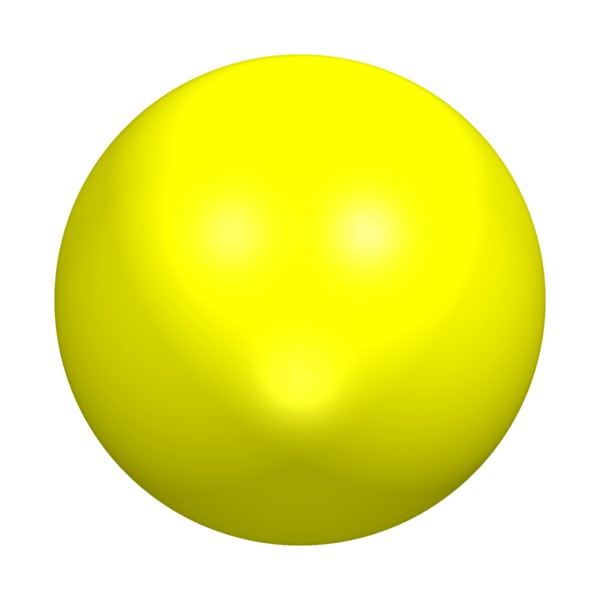
\includegraphics[width=1.1cm]{./../../common/images/kugel}
        \end{tabular}
        &
        \begin{tabular}{@{}c@{}}
          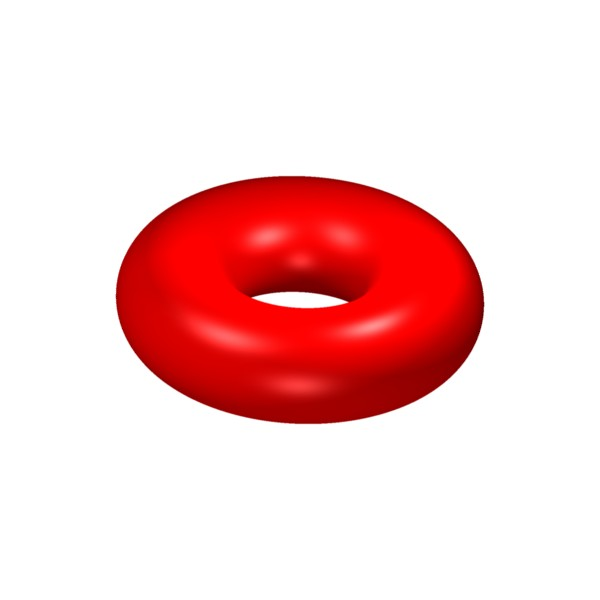
\includegraphics[width=1.1cm]{./../../common/images/torus}
        \end{tabular}
        &
        \begin{tabular}{@{}c@{}}
          많은\\
          특이점:
        \end{tabular}
        &
        \begin{tabular}{c@{}@{}}
          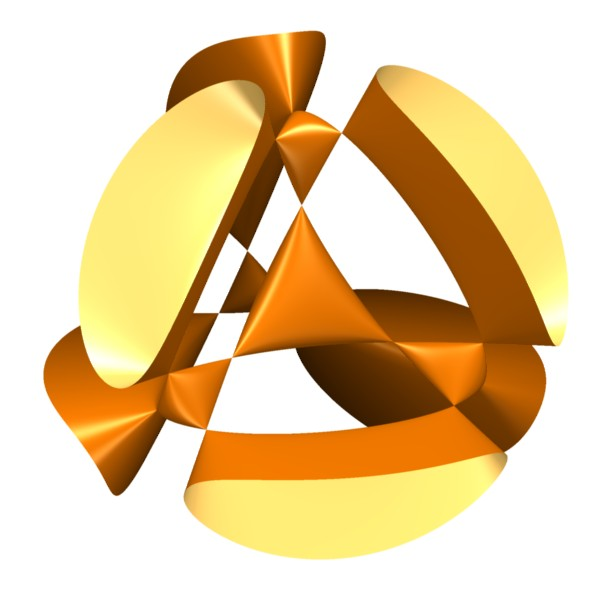
\includegraphics[width=1.1cm]{./../../common/images/kummer}
        \end{tabular}
        &
        \begin{tabular}{c@{}@{}}
          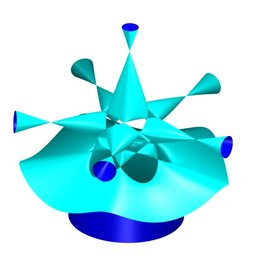
\includegraphics[width=1.1cm]{./../../common/images/togliatti}
        \end{tabular}
        &
        \begin{tabular}{c@{}@{}}
          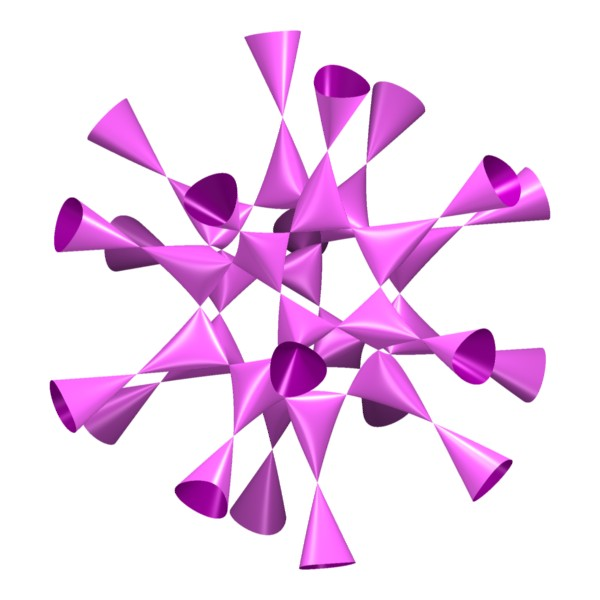
\includegraphics[width=1.1cm]{./../../common/images/barth_sextic}
        \end{tabular}
      \end{tabular}
    \end{center}
    \vspace{-0.2cm}
    곡면이 특이점을 갖는 것은 매우 특별한 상황입니다. SURFER 프로그램에서의 곡면들은 다항식으로부터 만들어집니다. 다항식의 가장 높은 지수 $d$를 이 다항식의 차수라고 합니다. 수학자들은 특정 차수의 다항식이 가질 수 있는 가장 많은 특이점의 갯수 대해 질문을 던져 왔습니다. 우리는 그 숫자를 $\mu(d)$ 라고 부릅니다.

$\mu(d)$ 는 계산하기 매우 어려운 숫자라는 것이 밝혀졌습니다. $19$세기에 $d=1,2,3,4$ 에 대해서는 밝혀졌지만 $d=5$ 에 대해서는 밝혀지지 않았습니다. $d=5$ 에 대해서는 1980년에 이르러서야 밝혀졌고, $d=6$ 에 대해서는 1996년에 밝혀졌습니다. $d=7$ 의 경우는 아직 미해결 문제입니다. 
  
그래서 $\mu(d)$에 대한 세계기록은 매우 중요한 결과입니다. 일반적인 $d$에 대해 완벽히 해결하기 위해서는 더 많은 시간이 소요될 것으로 보입니다. \\  다음은 몇가지 알려진 결과입니다.  
    
   \begin{center}
      \begin{tabular}{r|cccccccc|c}
        $d$ & $1$ & $2$ & $3$ & $4$ & $5$ & $6$ & $7$ & $8$ & $d$\\
        \hline
        \hline
        \rule{0pt}{1.2em}$\mu(d)\ge$ & $0$ & $1$ & $4$ & $16$ & $31$ & $65$ &
        $99$ & $168$ & 
        $\approx \frac{5}{12}d^3$\\[0.3em]
        \hline
        \rule{0pt}{1.2em}$\mu(d)\le$ & $0$ & $1$ & $4$ & $16$ & $31$ & $65$ &
        $104$ & $174$ & $\approx \frac{4}{9}d^3$
      \end{tabular}
    \end{center}
\end{surferIntroPage}
